\documentclass[border=10pt]{standalone}
\usepackage[svgnames]{xcolor}
\usepackage{amsmath}
\usepackage{pgfplots}
\pgfplotsset{compat=newest}
\usepackage[sfdefault]{FiraSans}
\usepackage{FiraMono}
\renewcommand*\familydefault{\sfdefault}
\begin{document}
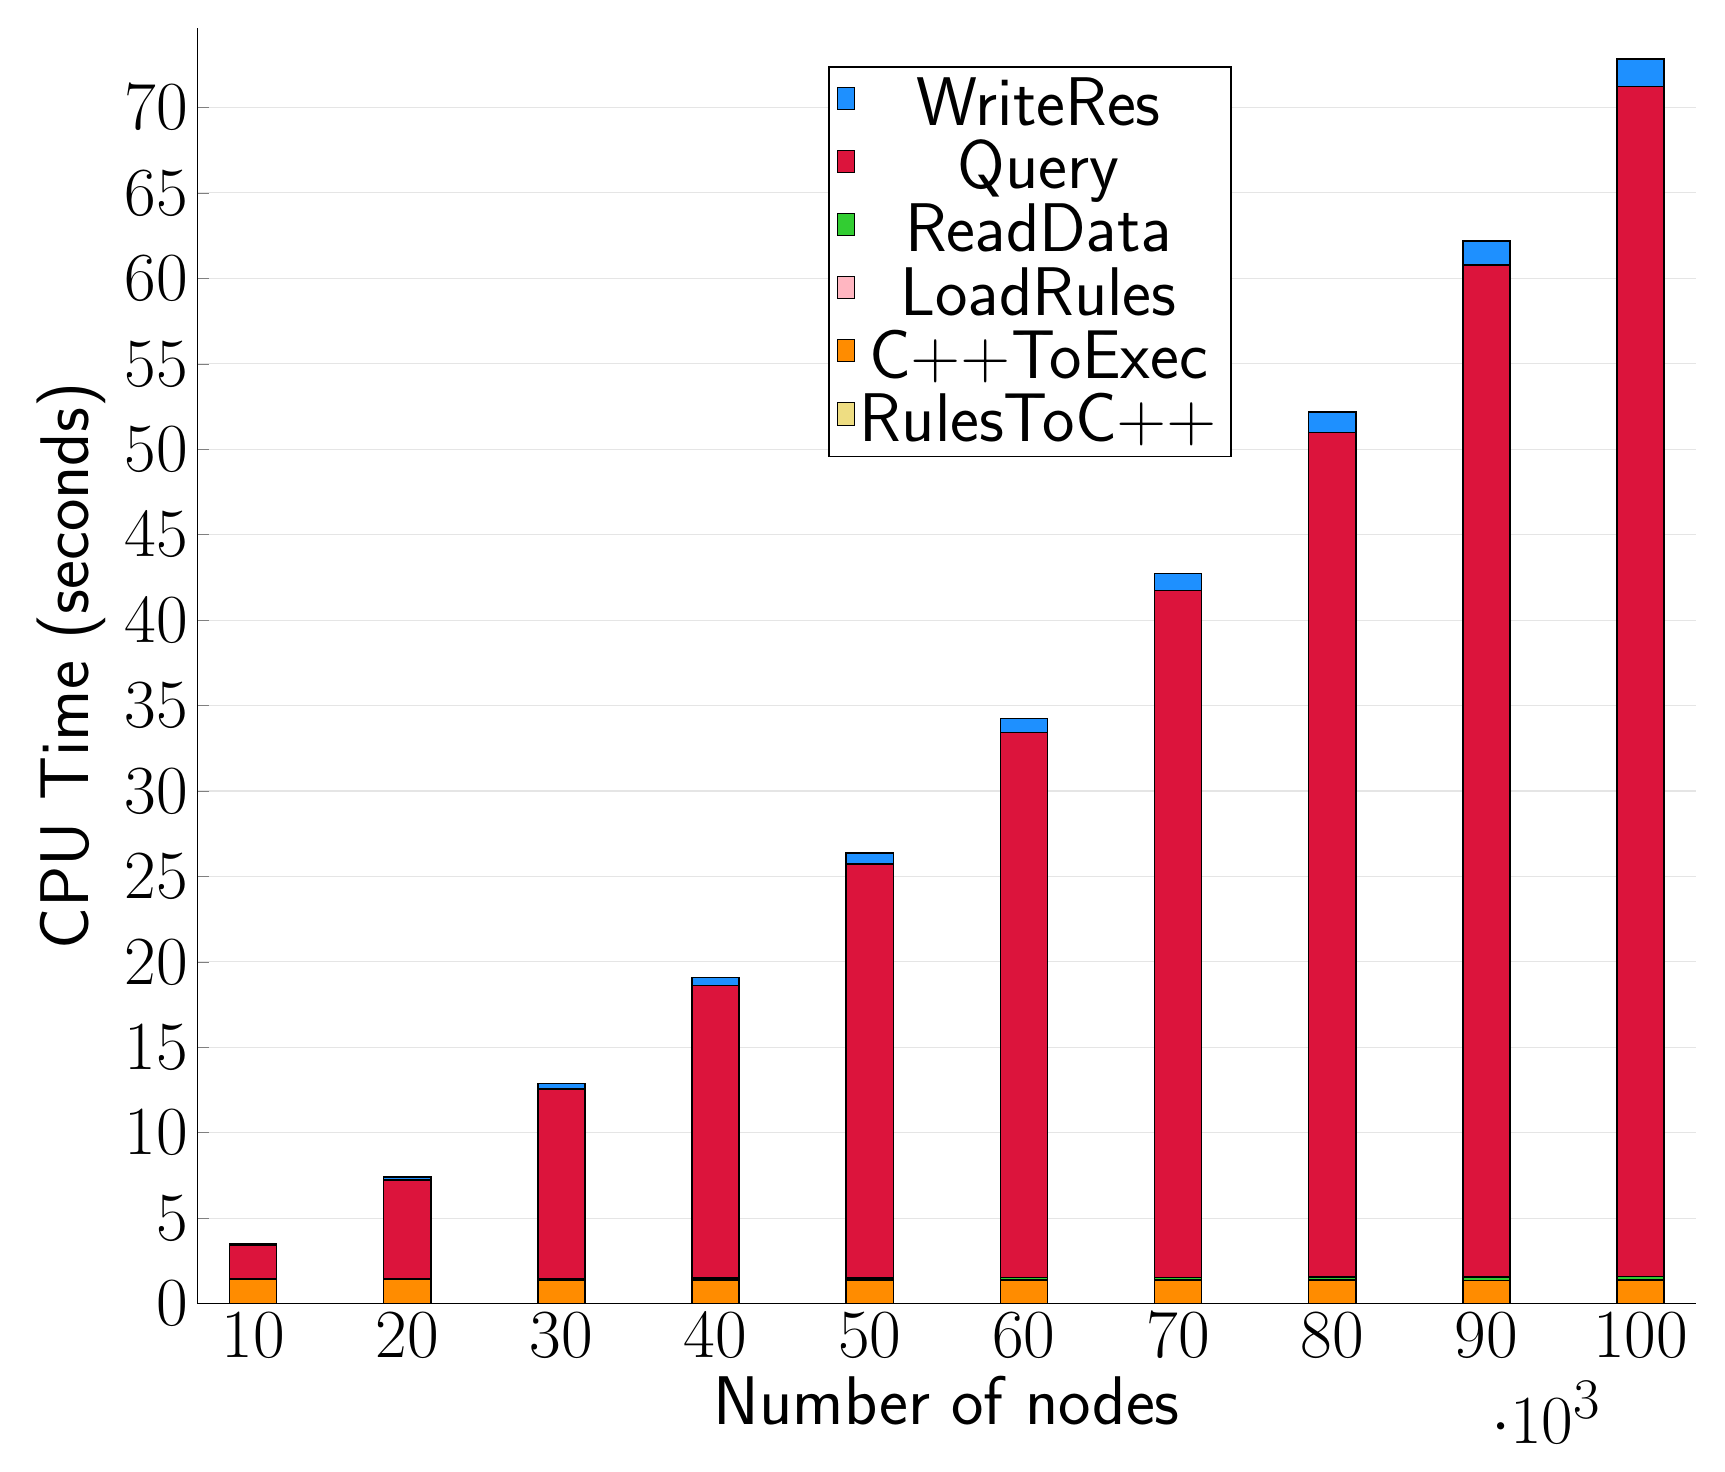
\begin{tikzpicture}
\begin{axis}[
   ybar stacked,
   width=1.7\textwidth,
   bar width=0.6cm,
   ymajorgrids, tick align=inside,
   major grid style={draw=gray!20},
   xtick=data,
   scaled x ticks={base 10:-3},
   ymin=0, ymax=74.64057999999999,
   axis x line*=bottom,
   axis y line*=left,
   enlarge x limits=0.04,
   legend style={
       at={(0.69, 0.97)},
       anchor=north east,
       legend columns=1,
       font=\Huge,
   },
   ylabel={CPU Time (seconds)},
   xlabel={Number of nodes},
   label style={font=\Huge},
   tick label style={font=\Huge},
]
\addlegendimage{fill=DodgerBlue, draw=black, line width=0.2pt}
\addlegendentry{WriteRes}
\addlegendimage{fill=Crimson, draw=black, line width=0.2pt}
\addlegendentry{Query}
\addlegendimage{fill=LimeGreen, draw=black, line width=0.2pt}
\addlegendentry{ReadData}
\addlegendimage{fill=LightPink, draw=black, line width=0.2pt}
\addlegendentry{LoadRules}
\addlegendimage{fill=DarkOrange, draw=black, line width=0.2pt}
\addlegendentry{C++ToExec}
\addlegendimage{fill=LightGoldenrod, draw=black, line width=0.2pt}
\addlegendentry{RulesToC++}
\addplot +[fill=LightGoldenrod, draw=black, line width=0.55pt] coordinates {
(10000, 0.006000000000000005)
(20000, 0.0)
(30000, 0.0020000000000000018)
(40000, 0.0020000000000000018)
(50000, 0.0)
(60000, 0.0)
(70000, 0.0)
(80000, 0.0)
(90000, 0.001999999999999999)
(100000, 0.001999999999999999)
};
\addplot +[fill=DarkOrange, draw=black, line width=0.55pt] coordinates {
(10000, 1.4080000000000001)
(20000, 1.3980000000000001)
(30000, 1.3820000000000001)
(40000, 1.3900000000000001)
(50000, 1.374)
(60000, 1.384)
(70000, 1.376)
(80000, 1.3719999999999999)
(90000, 1.3539999999999999)
(100000, 1.3639999999999999)
};
\addplot +[fill=LightPink, draw=black, line width=0.55pt] coordinates {
(10000, 0.00010140000000000001)
(20000, 8.779999999999999e-05)
(30000, 0.0001496)
(40000, 0.0001694)
(50000, 0.00016219999999999999)
(60000, 0.0001314)
(70000, 0.00013919999999999997)
(80000, 0.00012959999999999998)
(90000, 0.000134)
(100000, 0.00014360000000000002)
};
\addplot +[fill=LimeGreen, draw=black, line width=0.55pt] coordinates {
(10000, 0.028410599999999998)
(20000, 0.0529126)
(30000, 0.0733654)
(40000, 0.093247)
(50000, 0.1153424)
(60000, 0.1357042)
(70000, 0.1548332)
(80000, 0.172693)
(90000, 0.19390120000000002)
(100000, 0.210872)
};
\addplot +[fill=Crimson, draw=black, line width=0.55pt] coordinates {
(10000, 1.974306)
(20000, 5.77842)
(30000, 11.090019999999999)
(40000, 17.13158)
(50000, 24.2332)
(60000, 31.901400000000002)
(70000, 40.199940000000005)
(80000, 49.442620000000005)
(90000, 59.223580000000005)
(100000, 69.64057999999999)
};
\addplot +[fill=DodgerBlue, draw=black, line width=0.55pt] coordinates {
(10000, 0.0746878)
(20000, 0.1894566)
(30000, 0.32728340000000006)
(40000, 0.47760400000000003)
(50000, 0.6415980000000001)
(60000, 0.8222492000000001)
(70000, 1.0071292)
(80000, 1.2074840000000002)
(90000, 1.42036)
(100000, 1.62711)
};
\end{axis}
\end{tikzpicture}

\end{document}
